\documentclass{beamer} %[aspectratio=1610]

\usetheme{Darmstadt}
\usefonttheme[onlylarge]{structurebold}
\setbeamerfont*{frametitle}{size=\normalsize,series=\bfseries}
\setbeamertemplate{navigation symbols}{}

% Standard packages

\usepackage[english]{babel}
\usepackage[latin1]{inputenc}
\usepackage{times}
\usepackage[T1]{fontenc}
\usepackage{float}
\usepackage{graphicx}
\usepackage{subcaption}
\usepackage{ifthen}
\usepackage{minted}
\usepackage{verbatim}
%\usepackage{multimedia}
\usepackage[]{algorithm2e}

% Setup TikZ
\usepackage{tikz}
\usetikzlibrary{arrows}
\tikzstyle{block}=[draw opacity=0.7,line width=1.4cm]


% Author, Title, etc.
\title[Show me your properties! The potential of property-based testing in Agent-Based Simulation] 
{%
  Show me your properties! \\ The potential of property-based testing in Agent-Based Simulation
}

\author[Thaler]
{
  Jonathan~Thaler
}

\institute[University of Nottingham, Nottingham, United Kingdom]
{
  University of Nottingham, Nottingham, United Kingdom
}

\date[SummerSim'19, July 22-24, Berlin, Germany]
{SummerSim'19, July 22-24, Berlin, Germany}

% The main document

\begin{document}

\begin{frame}
  \titlepage
\end{frame}

\section{Introduction}
\begin{frame}{Testing in ABS?}
\begin{itemize}
	\item not existent, 1 paper focusing on it completely, very neglected but important. 
  	\item unit testing not very suitable for ABS in general?
  	\item lacking 
\end{itemize}

\begin{block}{}
Stochastic ABS + Randomised Property-Based Testing = $\heartsuit \heartsuit \heartsuit$
\end{block}
\end{frame}

\section{Property-Based Testing}
\begin{frame}{}
  \begin{itemize}
    \item Express specifications directly in code.
    \item QuickCheck library generates random test cases.
    \item Developer can express expected coverage.
    \item Part of the discovery and hypothesis process.
  \end{itemize}
\end{frame}

\begin{frame}[fragile]{QuickCheck}
\begin{block}{List Properties}
\begin{minted}[fontsize=\footnotesize]{haskell}
-- the reverse of a reversed list is the original list
reverse_reverse xs = reverse (reverse xs) == xs

-- concatenation operator (++) is associative
append_associative xs ys zs 
  = (xs ++ ys) ++ zs == xs ++ (ys ++ zs)

-- reverse is distributive over concatenation (++)
reverse_distributive xs ys 
  = reverse (xs ++ ys) == reverse xs ++ reverse ys
\end{minted}
\end{block}
\end{frame}

\begin{frame}[fragile]{QuickCheck cont'd}
\begin{block}{Running the tests...}
\begin{footnotesize}
\begin{verbatim}
+++ OK, passed 100 tests.
+++ OK, passed 100 tests.
*** Failed! Falsifiable (after 3 tests and 1 shrink):     
[1]
[0]
\end{verbatim}
\end{footnotesize}
\end{block}
\end{frame}

\begin{frame}[fragile]{QuickCheck cont'd}
\begin{block}{Labeling}
\begin{minted}[fontsize=\footnotesize]{haskell}
reverse_reverse_label xs  
  = label ("length of list is " ++ show (length xs)) 
          (reverse (reverse xs) == xs)
\end{minted}
\end{block}

\begin{block}{Running the tests...}
\begin{footnotesize}
\begin{verbatim}
+++ OK, passed 100 tests:
 5% length of list is 27
 5% length of list is 0
 4% length of list is 19
 ...
\end{verbatim}
\end{footnotesize}
\end{block}
\end{frame}

\begin{frame}[fragile]{QuickCheck cont'd}
\begin{block}{Coverage}
\begin{minted}[fontsize=\footnotesize]{haskell}
reverse_reverse_cover xs  = checkCoverage 
  cover 15 (length xs >= 50) "length of list at least 50"
  (reverse (reverse xs) == xs)
\end{minted}
\end{block}

\begin{block}{Running the tests...}
\begin{footnotesize}
\begin{verbatim}
+++ OK, passed 12800 tests 
    (15.445% length of list at least 50).
\end{verbatim}
\end{footnotesize}
\end{block}
\end{frame}

\section{Property-Based Testing in ABS}
\begin{frame}
\begin{block}{Randomised Property-Based Testing}
Matches the constructive and exploratory nature of ABS.
\end{block}

  \begin{itemize}
    \item Exploratory models: hypothesis tests about dynamics.
    \item Explanatory models: validate against formal specification.
    \item Test agent specification.
    \item Test simulation invariants.
  \end{itemize}
\end{frame}

\begin{frame}
\begin{block}{Randomised Property-Based Testing}
Matches the constructive and exploratory nature of ABS.
\end{block}

  \begin{itemize}
    \item Exploratory models: hypothesis tests about dynamics.
    \item Explanatory models: validate against formal specification.
    \item \textbf{Test agent specification.}
    \item \textbf{Test simulation invariants.}
  \end{itemize}
\end{frame}
  
\begin{frame}{Agent-Based SIR Model}
\begin{center}

\includegraphics[width=0.7\textwidth]{./fig/SIR_transitions.png}
\end{center}
  
  \begin{itemize}
    \item Population size $N = 1,000$
 	\item Contact rate $\beta = 5$
 	\item Infection probability $\gamma = 0.05$
 	\item Illness duration $\delta = 15$
 	\item 1 initially infected agent
  \end{itemize}
\end{frame}

\begin{frame}{Agent-Based SIR Dynamics}
\begin{center}
  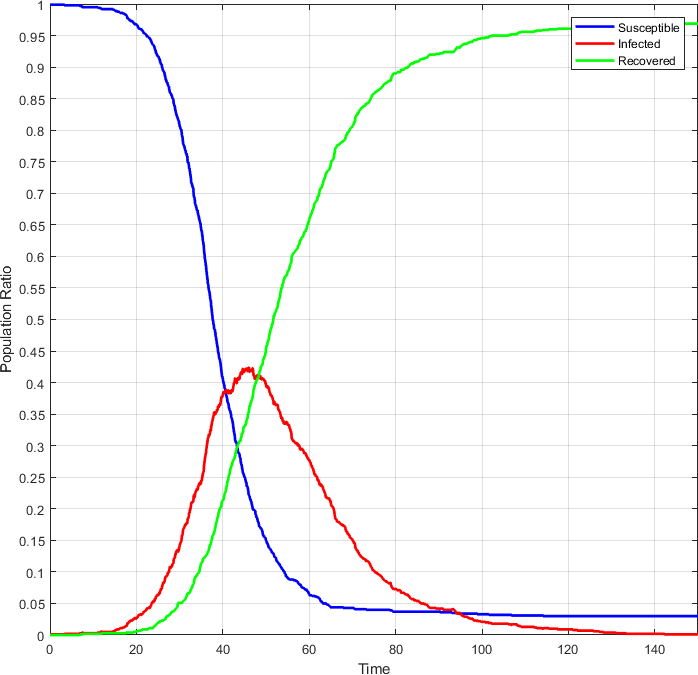
\includegraphics[width=0.7\textwidth]{./fig/SIR_Yampa_dt001.png}
\end{center}
\end{frame}

\begin{frame}{Test agent specification}
\begin{block}{Code / Implementation Testing}
Follow (formal) model specification / description.
\end{block}

\begin{block}{Examples}
  \begin{itemize}
    \item event-based: relate input to output events and perform random sampling
    \item time-based: encode invariants of output stream given random inputs
    \item use coverage to encode probabilities of e.g. transitions, timeouts,...
  \end{itemize}
\end{block}
\end{frame}

% TODO: go into detail of event-based and time-based

\begin{frame}{Agent-Based SIR Dynamics}
  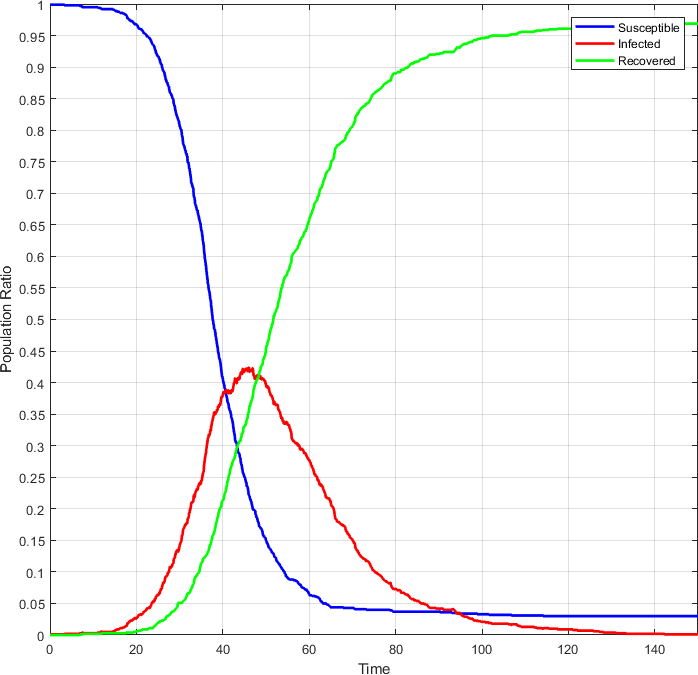
\includegraphics[width=0.7\textwidth]{./fig/SIR_Yampa_dt001.png}
\end{frame}

\begin{frame}{Test simulation invariants}
\begin{block}{Any Models}
Invariants have been established, fix them as test, used for regression testing.
\end{block}
\begin{block}{Example: agent-based SIR}
\begin{itemize}
	\item Time is monotonic decreasing
	\item Number of susceptible agents $S$ is monotonic decreasing.
	\item Number of recovered agents $R$ is monotonic increasing.
	\item Number of agents $N$ stays constant: N = S + I + R.
	\item Number of infected agents follows: I = N - (S + R).
\end{itemize}
\end{block}

\begin{block}{}
Property has to hold under random model parameters for all test cases, therefore no statistical testing.
\end{block}
\end{frame}

\begin{frame}[fragile]{Example: SIR invariants}
\begin{minted}[fontsize=\footnotesize]{haskell}
prop_sir_invariants :: Positive Int    -- ^ contact rate
                    -> Probability     -- ^ infectivity (0,1)
                    -> Positive Double -- ^ illness duration
                    -> TimeRange       -- ^ duration
                    -> [SIRState]      -- ^ population
                    -> Property
prop_sir_invariants 
    (Positive beta) (P gamma) (Positive delta) (T t) as  
  = property (do
    -- total agent count
    let n = length as
    -- run the SIR simulation with a new RNG 
    ret <- genSimulationSIR as beta gamma delta t
    -- check invariants and return result
    return (sirInvariants n ret)
\end{minted}
\end{frame}

\begin{frame}[fragile]{Example: SIR invariants}
\begin{minted}[fontsize=\tiny]{haskell}
sirInvariants :: Int                    -- ^ N total number of agents
              -> [(Time,(Int,Int,Int))] -- ^ output each step: (Time, (S,I,R))
              -> Bool
sirInvariants n aos = timeInc && aConst && susDec && recInc && infInv
  where
    (ts, sirs)  = unzip aos
    (ss, _, rs) = unzip3 sirs

    -- 1. time is monotonic increasing
    timeInc = allPairs (<=) ts
    -- 2. number of agents N stays constant in each step
    aConst = all agentCountInv sirs
    -- 3. number of susceptible S is monotonic decreasing
    susDec = allPairs (>=) ss
    -- 4. number of recovered R is monotonic increasing
    recInc = allPairs (<=) rs
    -- 5. number of infected I = N - (S + R)
    infInv = all infectedInv sirs

    agentCountInv :: (Int,Int,Int) -> Bool
    agentCountInv (s,i,r) = s + i + r == n

    infectedInv :: (Int,Int,Int) -> Bool
    infectedInv (s,i,r) = i == n - (s + r)

    allPairs :: (Ord a, Num a) => (a -> a -> Bool) -> [a] -> Bool
    allPairs f xs = all (uncurry f) (pairs xs)

    pairs :: [a] -> [(a,a)]
    pairs xs = zip xs (tail xs)
\end{minted}
\end{frame}

\section{Conclusions}
\begin{frame}{Conclusion}
	\begin{itemize}
		\item drawback: time consuming, sufficient coverage?
		\item deterministic: SmallCheck, enumerate test cases up to some given depth
	\end{itemize}
\end{frame}

\begin{frame}{}
  \begin{center}
  Thank You!
  \end{center}
\end{frame}

\bibliographystyle{acm}
\bibliography{../../writing/references/phdReferences.bib}

\end{document}